\chapter{oMdu kutUhala gaNita samaseyx}

namamx shAleya vijAcnxnakUTa ({\rm Science club}) na saBeyu kAyaR karxmada parxkAra ELu divasagaLagoMdu sala naDeyutitxtutx. kaLeda vArada vijAcnxnakekx saMbaMdhisida kAyaRkarxmavitutx. I sala nananx mitarx shArx e. veMkaTarAmf avarige AhAvxnisidedx. avaru utatxma gaNitajacnxru. avaru gaNitakekx saMbaMdhisidaMte yAvudAdarU kutUhala samaseyx heVLabeVkeMditutx. vijAcnxna kUTada sumAru ipapxteYdu sadasayxru sAmAnayxvAgi shanivAra beLagegx {\rm 10.30} gaMTege saBe seVrutitxdadxru.

AraMBadalilx sAvxgatada naMtara shArx e. veMkaTarAmf avaru sumAru hadineYdu rasaparxshenxgaLanunx keVLutatx sadasayxrige gaNitadalilx kutUhala mUDisidaru. anaMtara I citarxvanunx baredu
\begin{figure}[H]
\centering
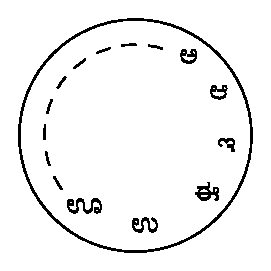
\includegraphics{src/figures/fig6.eps}
\end{figure}

ivugaLa parxtiVkaveVnu heVLi eMdaru.

a : - idu guNAkArada ananayxtA aMsha?

A : - idu paMcamAna padadhxtiya ati doDaDx aMke yAvudu?

i : - catuBuRjada oTuTx koVnagaLa motatx eSuTx laMbakoVnavAgirutatxde?

I : - eraDu ($2$) eMba saMKeyxya GanaveVnu?

u : - paMca BujAkaqtiyalilx eSuTx bAhugaLirutatxve?

U : - gArxmAMtara parxdeVshadalilx aLeyuvAga yAva I saMKeyxyanunx hecacxli (hecacxdu) enunxtAtxre?

I saMKeyxgaLanunx noVDidAga oMdu visheVSa saMKeyx eMdu gamanisabahudu. oMdanunx ($1$), $7$ eMba aviBAjayx saMKeyxyiMda BAgisidAga I saMKeyx doreyutatxde. yoVcisi nidhAnavAgi mADi eMdaru.

aSoTxtitxge oMdanunx, ELariMda BAgisidAga oMda saMKeyxyeV $142857 \ldots$ idu eMdaru.
$$
\frac{1}{7} = \cdot 142857 \ldots  
$$
\begin{multicols}{2}
\begin{figure}[H]
\centering
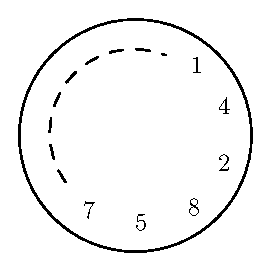
\includegraphics{src/figures/fig7.eps}
\end{figure}
\quad
\begin{tabular}{l@{\;}c@{\kern -4pt}l}
%  {l@{\;}c@{\kern -4pt}l}
$7$ & \Big) & ~~$10$ \Big($\cdot 142857$\\
&& ~~~\;$7$\\\cline{3-3}
&& ~~~\;$30$\\
&& ~~~\;$28$\\\cline{3-3}
&& ~~~~~\;$20$\\
&& ~~~~~\;$14$\\\cline{3-3}
&& ~~~~~~~\;$60$\\
  && ~~~~~~~\;$56$\\\cline{3-3}
  && ~~~~~~~~~\;$40$\\
  && ~~~~~~~~~\;$35$\\\cline{3-3}
  && ~~~~~~~~~~~\;$50$\\
  && ~~~~~~~~~~~\;$49$\\\cline{3-3}
  && ~~~~~~~~~~~~~\;$1$\\
  \end{tabular}
\end{multicols}

muMduvariyutatxde.
$$
{\text a} = 1, \quad {\text A} = 4, \quad {\text i} = 2, \quad {\text I} = 8, \quad {\text u} = 5, \quad {\text U} = 7
$$
AraMBadalilx baMdiruva biMdu ($\cdot$) biTuTxbiDi.

\newpage

$142857$ eMba saMKeyxyalilx matotxMdu visheVSa noVDabahudu nAneV heVLutetxVne keVLe. $142857$ nunx noVDi $1$ riMda $6$ ratanaka guNisidAga 
\begin{align*}
  142857 \times 1 & = 142857\\
  142857 \times 2 & = 285714\\
  142857 \times 3 & = 428571\\
  142857 \times 4 & =571428\\
  142857 \times 5 & =714285\\
  142857 \times 6 & =857142
\end{align*}
ivu cakirxyavAgi baMdive Adare oMdu mAlA saMKeyxyAgutetx aMdare $142857 \times 7 = 999.999$

